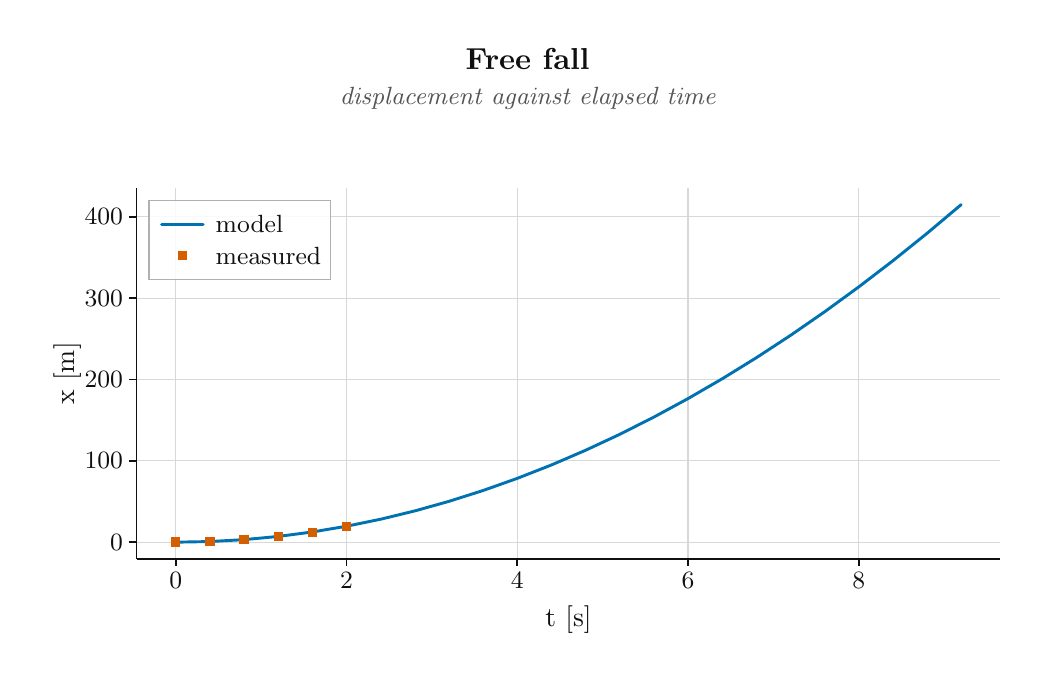
\begin{tikzpicture}[every node/.style={inner sep=0bp,outer sep=0bp}]
  \definecolor{qcA}{rgb}{1,1,1}
  \definecolor{qcB}{rgb}{0.062745,0.062745,0.062745}
  \definecolor{qcC}{rgb}{0.333333,0.333333,0.333333}
  \definecolor{qcD}{rgb}{0.847059,0.847059,0.847059}
  \definecolor{qcE}{rgb}{0,0.447059,0.698039}
  \def\quivermarkF#1#2{\path[fill,shift={(#1,#2)}] (-1.688bp,-1.688bp) rectangle (1.688bp,1.688bp);}
  \definecolor{qcG}{rgb}{0.835294,0.368627,0}
  \definecolor{qcH}{rgb}{0.690196,0.690196,0.690196}
  \useasboundingbox (0bp,0bp) rectangle (360bp,225bp);
  % quiver-key: figure
  \path[fill=qcA] (0bp,0bp) -- (360bp,0bp) -- (360bp,225bp) -- (0bp,225bp) -- cycle;
  % quiver-role: annotation -- Free fall
  \node[anchor=north,text=qcB,font=\bfseries\fontsize{11}{13.2}\selectfont] at (180bp,217.5bp) {Free fall};
  \node[anchor=north,text=qcC,font=\itshape\fontsize{9.5}{11.4}\selectfont] at (180bp,203.575bp) {displacement against elapsed time};
  % quiver-role: other:panel -- panel
  % quiver-data: row = 0
  % quiver-data: col = 0
  % quiver-data: layers = 2
  % quiver-data: x-tick-rule = all
  % quiver-data: y-tick-rule = all
  % quiver-role: decoration -- gridlines
  % quiver-data: lines = 10
  \path[draw=qcD,line width=0.375bp] (53.323bp,33.7bp) -- (53.323bp,167.375bp) (114.788bp,33.7bp) -- (114.788bp,167.375bp) (176.253bp,33.7bp) -- (176.253bp,167.375bp) (237.717bp,33.7bp) -- (237.717bp,167.375bp) (299.182bp,33.7bp) -- (299.182bp,167.375bp) (39.186bp,39.776bp) -- (350.198bp,39.776bp) (39.186bp,69.047bp) -- (350.198bp,69.047bp) (39.186bp,98.319bp) -- (350.198bp,98.319bp) (39.186bp,127.59bp) -- (350.198bp,127.59bp) (39.186bp,156.862bp) -- (350.198bp,156.862bp);
  \begin{scope}
    \clip (39.186bp,33.7bp) -- (350.198bp,33.7bp) -- (350.198bp,167.375bp) -- (39.186bp,167.375bp) -- cycle;
    % quiver-role: series -- model
    % quiver-data: series = model
    % quiver-data: points = 24
    \path[draw=qcE,line width=1.05bp,line cap=round,line join=round] (53.323bp,39.776bp) -- (65.616bp,40.006bp) -- (77.909bp,40.695bp) -- (90.202bp,41.844bp) -- (102.495bp,43.452bp) -- (114.788bp,45.519bp) -- (127.081bp,48.046bp) -- (139.374bp,51.032bp) -- (151.667bp,54.478bp) -- (163.96bp,58.384bp) -- (176.253bp,62.748bp) -- (188.546bp,67.572bp) -- (200.839bp,72.856bp) -- (213.132bp,78.599bp) -- (225.425bp,84.802bp) -- (237.717bp,91.463bp) -- (250.01bp,98.585bp) -- (262.303bp,106.166bp) -- (274.596bp,114.206bp) -- (286.889bp,122.706bp) -- (299.182bp,131.665bp) -- (311.475bp,141.083bp) -- (323.768bp,150.961bp) -- (336.061bp,161.299bp);
    % quiver-role: series -- measured
    % quiver-data: series = measured
    % quiver-data: points = 6
    \begin{scope}[fill=qcG]
      \quivermarkF{53.323bp}{39.776bp}
      \quivermarkF{65.616bp}{40.001bp}
      \quivermarkF{77.909bp}{40.675bp}
      \quivermarkF{90.202bp}{41.799bp}
      \quivermarkF{102.495bp}{43.373bp}
      \quivermarkF{114.788bp}{45.396bp}
    \end{scope}
  \end{scope}
  % quiver-role: axis -- t [s]
  % quiver-data: side = bottom
  % quiver-data: unit = s
  % quiver-data: prefix =
  % quiver-data: ticks = 5
  % quiver-data: tick-rule = all
  \path[draw=qcB,line width=0.6bp] (39.186bp,33.7bp) -- (350.198bp,33.7bp);
  \path[draw=qcB,line width=0.6bp] (53.323bp,33.7bp) -- (53.323bp,31.075bp) (114.788bp,33.7bp) -- (114.788bp,31.075bp) (176.253bp,33.7bp) -- (176.253bp,31.075bp) (237.717bp,33.7bp) -- (237.717bp,31.075bp) (299.182bp,33.7bp) -- (299.182bp,31.075bp);
  \node[anchor=north,text=qcB,font=\fontsize{9}{10.8}\selectfont] at (53.323bp,28.825bp) {0};
  \node[anchor=north,text=qcB,font=\fontsize{9}{10.8}\selectfont] at (114.788bp,28.825bp) {2};
  \node[anchor=north,text=qcB,font=\fontsize{9}{10.8}\selectfont] at (176.253bp,28.825bp) {4};
  \node[anchor=north,text=qcB,font=\fontsize{9}{10.8}\selectfont] at (237.717bp,28.825bp) {6};
  \node[anchor=north,text=qcB,font=\fontsize{9}{10.8}\selectfont] at (299.182bp,28.825bp) {8};
  \node[anchor=north,text=qcB,font=\fontsize{10}{12}\selectfont] at (194.692bp,16.75bp) {t [s]};
  % quiver-role: axis -- x [m]
  % quiver-data: side = left
  % quiver-data: unit = m
  % quiver-data: prefix =
  % quiver-data: ticks = 5
  % quiver-data: tick-rule = all
  \path[draw=qcB,line width=0.6bp] (39.186bp,33.7bp) -- (39.186bp,167.375bp);
  \path[draw=qcB,line width=0.6bp] (39.186bp,39.776bp) -- (36.561bp,39.776bp) (39.186bp,69.047bp) -- (36.561bp,69.047bp) (39.186bp,98.319bp) -- (36.561bp,98.319bp) (39.186bp,127.59bp) -- (36.561bp,127.59bp) (39.186bp,156.862bp) -- (36.561bp,156.862bp);
  \node[anchor=east,text=qcB,font=\fontsize{9}{10.8}\selectfont] at (34.311bp,39.776bp) {0};
  \node[anchor=east,text=qcB,font=\fontsize{9}{10.8}\selectfont] at (34.311bp,69.047bp) {100};
  \node[anchor=east,text=qcB,font=\fontsize{9}{10.8}\selectfont] at (34.311bp,98.319bp) {200};
  \node[anchor=east,text=qcB,font=\fontsize{9}{10.8}\selectfont] at (34.311bp,127.59bp) {300};
  \node[anchor=east,text=qcB,font=\fontsize{9}{10.8}\selectfont] at (34.311bp,156.862bp) {400};
  \node[anchor=base,text=qcB,rotate=90,font=\fontsize{10}{12}\selectfont] at (16.75bp,100.537bp) {x [m]};
  % quiver-role: legend -- legend
  % quiver-data: entries = 2
  \path[fill=qcA,fill opacity=0.85,draw=qcH,line width=0.45bp] (43.686bp,134.225bp) -- (108.999bp,134.225bp) -- (108.999bp,162.875bp) -- (43.686bp,162.875bp) -- cycle;
  % quiver-role: other:legend-entry -- model
  % quiver-data: series = model
  % quiver-data: color = #0072b2
  \path[draw=qcE,line width=1.05bp,line cap=round] (48.186bp,154.212bp) -- (63.186bp,154.212bp);
  \node[anchor=west,text=qcB,font=\fontsize{9}{10.8}\selectfont] at (67.686bp,154.212bp) {model};
  % quiver-role: other:legend-entry -- measured
  % quiver-data: series = measured
  % quiver-data: color = #d55e00
  \begin{scope}[fill=qcG]
    \quivermarkF{55.686bp}{142.887bp}
  \end{scope}
  \node[anchor=west,text=qcB,font=\fontsize{9}{10.8}\selectfont] at (67.686bp,142.887bp) {measured};
\end{tikzpicture}
